\documentclass[12pt]{report}

\usepackage{mathtools}
\usepackage{MnSymbol}
\usepackage[section]{placeins}
\usepackage{multirow}
\usepackage{pifont}
\usepackage[top=3cm,right=3cm,bottom=3cm,left=3cm]{geometry}
\usepackage{indentfirst}
\usepackage{graphicx}
\usepackage{rotating}
\usepackage{subcaption}
\usepackage[usenames,dvipsnames]{color,xcolor}
\usepackage{pgf}
\usepackage{colortbl}
\usepackage{listings}
\usepackage{cite}
\usepackage{tikz}
\newcommand*\circled[1]{
	\tikz[baseline=(char.base)]{
		\node[shape=circle,draw,inner sep=-4pt] (char) {#1\strut}
	}\kern-3pt
}
\usepackage{accents}
\newcommand{\ubar}[1]{\underaccent{\bar}{#1}}
\usepackage{matlab-prettifier}
\usepackage[colorlinks,linkcolor=blue,citecolor=red]{hyperref}
\usepackage{fancyhdr}
\usepackage{amsmath}
\usepackage{xepersian}
%\settextfont{B Nazanin}
\settextfont{XB Niloofar.ttf}
\setdigitfont{XB Niloofar.ttf}
\linespread{1.7}
\usepackage[perpage]{footmisc}


\geometry{letterpaper, portrait, includeheadfoot=true, hmargin=1in, vmargin=1in}


\begin{document}
	\renewcommand{\familydefault}{\rmdefault}
	
	\begin{titlepage}
    \begin{center}
    \begin{figure}
        \centering
        
\includegraphics[width=0.5\linewidth]{KNTU.png}
    \end{figure}

    {\fontsize{24}{32}\selectfont \bfseries آنالیز ریسک در سیستم حمل و نقل عمومی} 
    \\\vspace{20pt}
    دانشجو:\\
    {\LARGE علی شریفی} \\
    \vspace{10pt}
    \textbf{40114494}\\
    \vspace{20pt}
    استاد درس:\\
    {\LARGE دکتر احمدرضا تحسیری} \\
    \vfill
    تابستان 1403
    \end{center}

\end{titlepage}
	\begin{abstract}
این پروژه به تحلیل ریسک سیستم حمل و نقل عمومی از طریق روشهای تحلیل درخت خطا (FTA) می‌پردازد. هدف از این مطالعه، شناسایی و ارزیابی عوامل ریسک زا و ریسک پذیر در سیستم حمل و نقل عمومی و ارائه راهکارهایی برای کاهش این ریسک‌هاست. ابتدا سیستم حمل و نقل عمومی مورد بررسی قرار می‌گیرد و عوامل مختلفی نظیر خرابی وسایل نقلیه، نگهداری نامناسب، کمبود نیروی کار ماهر، آموزش ناکافی کارکنان، برنامه‌ریزی ناکارآمد مسیرها و شرایط آب و هوایی نامناسب به عنوان رویدادهای ابتدایی شناسایی می‌شوند. سپس با استفاده از تحلیل درخت خطا (FTA)، ارتباطات منطقی بین این رویدادها و رویداد اصلی (توقف کامل سیستم حمل و نقل) تحلیل و به صورت نمودار درخت خطا ترسیم می‌شود. نتایج این تحلیل‌ها می‌تواند به مدیران و مسئولان کمک کند تا نقاط ضعف سیستم را شناسایی کرده و با اتخاذ تدابیر مناسب، کارایی و پایداری سیستم حمل و نقل عمومی را بهبود بخشند.
	\end{abstract}
	\pagestyle{fancy}
\fancyhead{}
\fancyfoot{}
\fancyhead[C]{\leftmark}
\fancyfoot[C]{\thepage}
\pagestyle{fancy}
	\pagenumbering{alph}
	\tableofcontents
	\listoffigures
	\addcontentsline{toc}{chapter}{فهرست تصاویر}
	\pagebreak
	
	\chapter{مقدمه}
\pagenumbering{arabic}
سیستم حمل و نقل عمومی از اجزای حیاتی زیرساخت‌های شهری است که نقش کلیدی در بهبود کیفیت زندگی شهروندان ایفا می‌کند. این سیستم با ارائه خدمات جابجایی امن، کارآمد، و مقرون به صرفه به میلیون‌ها نفر در سراسر جهان کمک می‌کند تا به محل کار، تحصیل، و دیگر مقاصد خود برسند. حمل و نقل عمومی نه تنها به کاهش تراکم ترافیک و آلودگی هوا کمک می‌کند، بلکه به افزایش بهره‌وری اقتصادی و دسترسی بیشتر به فرصت‌های اجتماعی و اقتصادی نیز منجر می‌شود\cite{beirao2007}.


سیستم حمل و نقل عمومی از چندین جزء اصلی تشکیل شده است که هر یک نقشی اساسی در عملکرد کلی آن دارند. این اجزا شامل وسایل نقلیه (مانند اتوبوس‌ها، متروها، ترامواها و تاکسی‌ها)، زیرساخت‌ها (مانند ایستگاه‌ها، خطوط ریلی و مسیرهای اتوبوس)، و سیستم‌های پشتیبانی (مانند سیستم‌های بلیت‌فروشی، مدیریت ترافیک و مراکز تعمیر و نگهداری) می‌شود.


علی‌رغم مزایای فراوان، سیستم‌های حمل و نقل عمومی با چالش‌های متعددی نیز مواجه هستند. از جمله این چالش‌ها می‌توان به نیاز به تعمیر و نگهداری مستمر، تأمین مالی پایدار، مقابله با حوادث و بلایای طبیعی، و جلب رضایت مسافران اشاره کرد. با این حال، فرصت‌های بسیاری نیز برای بهبود و توسعه این سیستم‌ها وجود دارد. به‌کارگیری فناوری‌های پاک و پایدار، توسعه شبکه‌های حمل و نقل، و افزایش همکاری‌های بین‌المللی از جمله راهکارهایی هستند که می‌توانند به ارتقای سیستم‌های حمل و نقل عمومی کمک کنند.
	\chapter{تحلیل سیستم و شناسایی اجزا}
\section{تحلیل سیستم حمل و نقل عمومی و شناسایی اجزا}

تحلیل سیستم حمل و نقل عمومی شامل شناسایی و بررسی دقیق اجزای مختلف این سیستم و چگونگی تعامل آن‌ها با یکدیگر است. این تحلیل به ما کمک می‌کند تا عملکرد کلی سیستم را بهبود دهیم و مشکلات را شناسایی و حل کنیم. در این بخش، به تفصیل اجزای کلیدی سیستم حمل و نقل عمومی و نقش هر یک از این اجزا را بررسی خواهیم کرد.

\section{وسیله‌های نقلیه عمومی}
وسایل نقلیه عمومی شامل اتوبوس‌ها، متروها، قطارها، ترامواها و تاکسی‌ها هستند که هر یک نقش مهمی در جابجایی مسافران دارند. ویژگی‌های کلیدی این وسایل نقلیه عبارتند از:

\textbf{ظرفیت حمل و نقل:}
 تعداد مسافرانی که وسیله نقلیه می‌تواند در هر سفر حمل کند.
 
\textbf{زمان‌بندی و فرکانس:}
تعداد دفعات حرکت وسیله نقلیه در طول روز و دقت زمانی در اجرای این برنامه.

\textbf{راحتی و امنیت:}
کیفیت خدمات ارائه شده به مسافران و میزان امنیت در طول سفر.

\section{ایستگاه‌ها و پایانه‌ها}
ایستگاه‌ها و پایانه‌ها نقاط کلیدی برای سوار و پیاده شدن مسافران هستند و شامل:

\textbf{ایستگاه‌های اتوبوس:}
محل‌هایی که اتوبوس‌ها در آن توقف می‌کنند تا مسافران سوار یا پیاده شوند.

\textbf{ایستگاه‌های مترو و قطار:}
شامل سکوها، ورودی‌ها و خروجی‌ها و امکانات رفاهی برای مسافران.

\textbf{پایانه‌های حمل و نقل:}
نقاط تجمیع وسایل نقلیه مختلف که امکان تعویض وسیله نقلیه را برای مسافران فراهم می‌کنند.

\section{زیرساخت‌های فیزیکی}
زیرساخت‌های فیزیکی شامل جاده‌ها، خطوط ریلی، تونل‌ها و پل‌ها هستند که وسایل نقلیه از آن‌ها استفاده می‌کنند. این زیرساخت‌ها باید:
- **با کیفیت بالا و قابل اطمینان**: برای کاهش خرابی‌ها و تأخیرها.
- **ایمن**: برای جلوگیری از حوادث و تصادفات.
- **مناسب برای همه اقشار جامعه**: به منظور دسترسی آسان برای افراد با نیازهای خاص.

\section{سیستم‌های اطلاعاتی و فناوری}
سیستم‌های اطلاعاتی و فناوری نقش مهمی در بهبود عملکرد و کارایی سیستم حمل و نقل عمومی دارند و شامل:

\textbf{سیستم‌های مدیریت ترافیک:}
برای کنترل و هدایت جریان ترافیک و کاهش ازدحام.

\textbf{سیستم‌های پرداخت الکترونیکی:}
برای ساده‌سازی فرایند خرید بلیت و افزایش راحتی مسافران.

\textbf{سیستم‌های اطلاع‌رسانی به مسافران:}
شامل نمایشگرهای دیجیتال و اپلیکیشن‌های موبایل برای ارائه اطلاعات لحظه‌ای در مورد زمان‌بندی و مسیرها.

\section{نیروی انسانی}
نیروی انسانی شامل رانندگان، نگهبانان، کارکنان تعمیر و نگهداری و پرسنل مدیریت است. ویژگی‌های کلیدی نیروی انسانی عبارتند از:

\textbf{مهارت و آموزش:}
کارکنان باید دارای مهارت‌های لازم و آموزش‌های کافی برای انجام وظایف خود باشند.

\textbf{رضایت شغلی و شرایط کاری مناسب:}
برای افزایش بهره‌وری و کاهش ترک خدمت.



	\chapter{شناسایی و تحلیل ریسک‌ها}

شناسایی و تحلیل ریسک‌ها در سیستم حمل و نقل عمومی یک فرآیند حیاتی برای اطمینان از عملکرد بهینه و ایمن این سیستم است. این فرآیند به شناسایی، ارزیابی و اولویت‌بندی ریسک‌هایی می‌پردازد که می‌توانند بر عملکرد و ایمنی سیستم حمل و نقل تأثیر بگذارند. در ادامه، این فرآیند به طور مفصل تشریح می‌شود\cite{charnes1978}.

\section{شناسایی ریسک‌ها}
شناسایی ریسک‌ها اولین گام در تحلیل ریسک است و شامل شناسایی کلیه عواملی است که می‌توانند به هر نحوی عملکرد سیستم حمل و نقل عمومی را تحت تأثیر قرار دهند. این ریسک‌ها به دو دسته اصلی تقسیم می‌شوند: ریسک‌های داخلی و ریسک‌های محیطی.

\subsection{ریسک‌های داخلی}
\begin{enumerate}
	\item \textbf{مشکلات فنی و نگهداری}
	\begin{itemize}
		\item \textbf{خرابی وسایل نقلیه}: مشکلات مکانیکی یا الکتریکی در اتوبوس‌ها، متروها و قطارها که می‌تواند منجر به توقف یا تأخیر در خدمات شود. به عنوان مثال، خرابی موتور یا سیستم ترمز.
		\item \textbf{نگهداری نامناسب}: عدم انجام به‌موقع تعمیرات و نگهداری منظم که می‌تواند عمر مفید وسایل نقلیه را کاهش دهد و خطرات ایمنی ایجاد کند.
	\end{itemize}
	\item \textbf{مدیریت و منابع انسانی}
	\begin{itemize}
		\item \textbf{کمبود نیروی کار ماهر}: کمبود رانندگان و تکنسین‌های ماهر که می‌تواند به کاهش کیفیت خدمات و افزایش خطرات ایمنی منجر شود.
		\item \textbf{آموزش ناکافی کارکنان}: عدم ارائه آموزش‌های کافی به کارکنان در زمینه‌های ایمنی، خدمات مشتری و عملیات سیستم که می‌تواند کارایی را کاهش داده و خطرات را افزایش دهد.
	\end{itemize}
	\item \textbf{کارایی عملیاتی}
	\begin{itemize}
		\item \textbf{برنامه‌ریزی ناکارآمد مسیرها}: برنامه‌ریزی نامناسب مسیرها و زمان‌بندی‌ها که می‌تواند به تأخیرها، ازدحام و نارضایتی مسافران منجر شود.
		\item \textbf{ظرفیت ناکافی}: ناتوانی در پاسخ به تقاضای مسافران در ساعات اوج که می‌تواند به ازدحام و نارضایتی مسافران منجر شود.
	\end{itemize}
	\item \textbf{امنیت}
	\begin{itemize}
		\item \textbf{جرم و جنایت}: وقوع جرم و جنایت در ایستگاه‌ها و وسایل نقلیه که می‌تواند به کاهش احساس امنیت و نارضایتی مسافران منجر شود.
		\item \textbf{عدم آمادگی برای حوادث اضطراری}: ناتوانی در پاسخ به حوادث اضطراری مانند آتش‌سوزی یا حملات تروریستی که می‌تواند به خطرات جانی و مالی جدی منجر شود.
	\end{itemize}
\end{enumerate}

\subsection{ریسک‌های محیطی}
\begin{enumerate}
	\item \textbf{عوامل اقتصادی}
	\begin{itemize}
		\item \textbf{نوسانات قیمت سوخت}: تغییرات در قیمت سوخت که می‌تواند به افزایش هزینه‌های عملیاتی منجر شود.
		\item \textbf{وضعیت اقتصادی کلان}: رکود اقتصادی که می‌تواند به کاهش بودجه‌های دولتی و کاهش تقاضای حمل و نقل عمومی منجر شود.
	\end{itemize}
	\item \textbf{عوامل اجتماعی}
	\begin{itemize}
		\item \textbf{تغییرات جمعیتی}: تغییرات در جمعیت و توزیع جغرافیایی مسافران که می‌تواند به تغییر در تقاضا برای خدمات حمل و نقل منجر شود.
		\item \textbf{تغییر در الگوهای سفر}: تغییر در الگوهای کاری و زندگی که می‌تواند به تغییر در نیازهای حمل و نقل عمومی منجر شود.
	\end{itemize}
	\item \textbf{عوامل سیاسی و قانونی}
	\begin{itemize}
		\item \textbf{تغییرات در سیاست‌های دولتی}: تغییر در قوانین و مقررات که می‌تواند به تأثیرات مالی و عملیاتی برای سیستم حمل و نقل منجر شود.
		\item \textbf{نوسانات در حمایت‌های دولتی}: تغییرات در میزان و نوع حمایت‌های دولتی که می‌تواند به تغییر در بودجه‌ها و منابع مالی منجر شود.
	\end{itemize}
	\item \textbf{عوامل طبیعی و محیطی}
	\begin{itemize}
		\item \textbf{شرایط آب و هوایی نامناسب}: شرایط آب و هوایی شدید مانند برف، باران شدید یا طوفان که می‌تواند به تأخیرها و لغو خدمات منجر شود.
		\item \textbf{بلایای طبیعی}: وقوع بلایای طبیعی مانند زلزله، سیل یا آتش‌سوزی که می‌تواند به خرابی زیرساخت‌ها و وسایل نقلیه منجر شود.
	\end{itemize}
\end{enumerate}


\section{تجزیه و تحلیل درخت خطا (FTA) در سیستم حمل و نقل عمومی}

درخت خطا (\lr{Fault Tree Analysis}) یک روش گرافیکی و سیستماتیک برای تحلیل عوامل و رویدادهایی است که می‌توانند منجر به وقوع یک حادثه یا خرابی خاص در یک سیستم شوند. در تحلیل درخت خطا، رویدادهای ابتدایی (\lr{Basic Events}) که می‌توانند به یک رویداد اصلی (\lr{Top Event}) منجر شوند، شناسایی و تحلیل می‌شوند. این روش به شناسایی نقاط ضعف سیستم و تعیین راهکارهای پیشگیرانه کمک می‌کند.

\subsection{ساختار درخت خطا}

ساختار درخت خطا شامل یک نمودار درختی است که مسیرهای مختلفی را که می‌توانند منجر به وقوع یک حادثه خاص شوند، نشان می‌دهد. این نمودار از رویدادهای ابتدایی به سمت رویداد اصلی هدایت می‌شود. در ادامه، مراحل ساختار درخت خطا برای سیستم حمل و نقل عمومی را توضیح می‌دهیم.

\subsubsection{شناسایی رویداد اصلی}

رویداد اصلی (\lr{Top Event}) در تحلیل درخت خطا، حادثه یا خرابی اصلی است که می‌خواهیم از وقوع آن جلوگیری کنیم. در سیستم حمل و نقل عمومی، رویداد اصلی می‌تواند "توقف کامل سیستم حمل و نقل" باشد.

\subsubsection{شناسایی رویدادهای ابتدایی}

رویدادهای ابتدایی (\lr{Basic Events}) رویدادهایی هستند که به وقوع رویداد اصلی منجر می‌شوند. این رویدادها می‌توانند شامل عوامل فنی، مدیریتی، انسانی و محیطی باشند. برخی از رویدادهای ابتدایی در سیستم حمل و نقل عمومی عبارتند از:

\begin{itemize}
	\item خرابی وسایل نقلیه ($ V_1 $)
	\item نگهداری نامناسب ($ V_2 $)
	\item کمبود نیروی کار ماهر ($ H_1 $)
	\item آموزش ناکافی کارکنان ($ H_2 $)
	\item برنامه‌ریزی ناکارآمد مسیرها ($ O_1 $)
	\item شرایط آب و هوایی نامناسب ($ E_1 $)
\end{itemize}

\subsubsection{نمودار درخت خطا}

نمودار درخت خطا برای رویداد اصلی "توقف کامل سیستم حمل و نقل عمومی" به صورت زیر ترسیم می‌شود.
\begin{figure}[!ht]
	\centering
	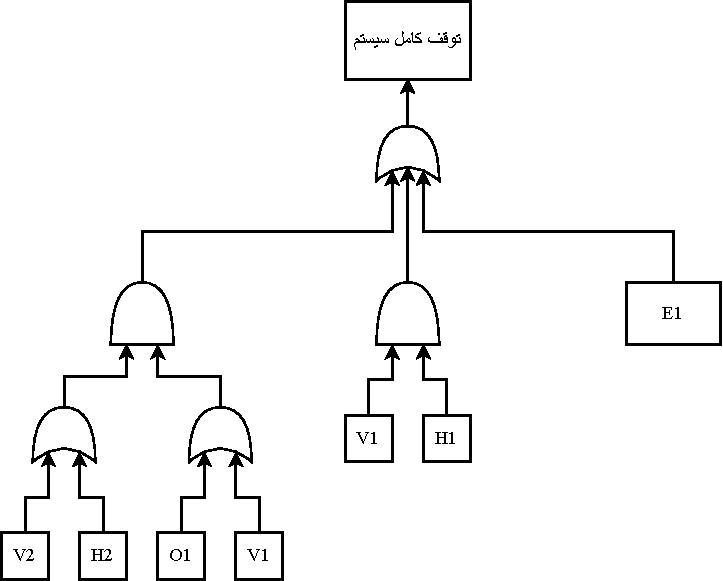
\includegraphics[width=0.5\linewidth]{fig/fig1.pdf}
	\caption{درخت خطای مربوط به سیستم حمل و نقل عمومی}
\end{figure}

\section{مدلسازی ریاضی}
با توجه به درخت خطا، مدل ریاضی به صورت زیر به دست می‌آید،
\begin{equation}
	1 - \left[1-\left[1-\left(1-X_1\right)\left(1-X_2\right)\right] \left[1-\left(1-X_3\right)\left(1-X_4\right)\right]\right] \left[1-X_4X_5\right] \left[1-X_6\right],
\end{equation}
که متغیرهای موجود در این عبارت ریاضی به صورت زیر نعریف شده‌اند،
\begin{itemize}
	\item $X_1$: نگهداری نامناسب
	\item $X_2$: آموزش ناکافی کارکنان
	\item $X_3$: برنامه‌ریزی ناکارآمد مسیرها
	\item $X_4$: خرابی وسایل نقلیه
	\item $X_5$: کمبود نیروی کار ماهر
	\item $X_6$: شرایط آب ‌و هوایی نامناسب
\end{itemize}
	\chapter{نتیجه‌گیری}
در این پروژه به بررسی و تحلیل ریسک‌های سیستم حمل و نقل عمومی از طریق روش‌های تحلیل درخت خطا (FTA) پرداخته شد. هدف اصلی این مطالعه شناسایی و ارزیابی عوامل ریسک زا و ریسک پذیر در سیستم حمل و نقل عمومی و ارائه راهکارهایی برای کاهش این ریسک‌ها بود. 
رویداد اصلی در این درخت خطا، "توقف کامل سیستم حمل و نقل" تعیین شد. عوامل مختلفی نظیر خرابی وسایل نقلیه، نگهداری نامناسب، کمبود نیروی کار ماهر، آموزش ناکافی کارکنان، برنامهریزی ناکارآمد مسیرها، و شرایط آب و هوایی نامناسب به عنوان رویدادهای ابتدایی شناسایی شدند. نمودار درخت خطا ترسیم شد که ارتباطات منطقی بین این رویدادها و رویداد اصلی را نمایش می‌داد. این تحلیل به شناسایی نقاط ضعف سیستم و ارائه راهکارهای پیشگیرانه کمک کرد.

\section{پیشنهادات برای بهبود}

با توجه به نتایج به دست آمده از تحلیلهای FTA، پیشنهادات زیر برای بهبود سیستم حمل و نقل عمومی ارائه میشود:

\subsection{بهبود نگهداری و تعمیرات:}
- تدوین و اجرای برنامههای نگهداری و تعمیرات پیشگیرانه برای کاهش احتمال خرابی وسایل نقلیه.
- استفاده از فناوریهای نوین برای پایش و مدیریت وضعیت وسایل نقلیه.

\subsection{آموزش و توسعه نیروی کار:}
- برگزاری دورههای آموزشی منظم و کاربردی برای کارکنان به منظور افزایش مهارتها و دانش فنی.
- استخدام و حفظ نیروی کار ماهر با ارائه انگیزهها و امکانات مناسب.

\subsection{برنامهریزی کارآمد:}
- بهبود فرآیندهای برنامهریزی مسیرها و زمانبندی سفرها برای افزایش کارایی و کاهش تأخیرات.
- استفاده از سیستمهای مدیریت هوشمند ترافیک برای بهینهسازی مسیرها و کاهش زمان سفر.

\subsection{مدیریت شرایط محیطی:}
- توسعه و اجرای برنامههای مدیریت بحران برای مواجهه با شرایط آب و هوایی نامناسب.
- ارتقاء زیرساختها برای افزایش مقاومت سیستم در برابر شرایط نامطلوب جوی.


این پروژه نشان داد که تحلیل ریسک با استفاده از روش FTA می‌تواند به شناسایی و ارزیابی نقاط ضعف و قوت سیستم حمل و نقل عمومی کمک کند. با بهره‌گیری از این تحلیل‌ها و اجرای راهکارهای پیشنهادی، می‌توان کارایی و پایداری سیستم حمل و نقل عمومی را بهبود بخشید و ریسک‌های مرتبط با آن را به حداقل رساند.
	\input{conclusion}
	
	\bibliographystyle{ieeetr-fa}
	\bibliography{reference}
	\addcontentsline{toc}{chapter}{کتاب‌نامه}
\end{document}
